% \documentclass[english, draft]{article}
\documentclass[english]{article}

%\usepackage[showframe]{geometry}
\usepackage{geometry}
\usepackage{float}
\usepackage[utf8]{inputenc}
\usepackage[backend=biber,style= authoryear]{biblatex}
% \usepackage[backend=biber]{biblatex}
\usepackage[english]{babel}
\usepackage{csquotes}
\usepackage{graphicx}
\usepackage{subcaption}
\usepackage{booktabs}

\usepackage{xargs}
\usepackage[pdftex,dvipsnames,table]{xcolor}

\graphicspath{{./resources/images}}
\addbibresource{../articles.bib}
\addbibresource{../manual.bib}

\geometry{a4paper, total={165mm,257mm}, left=15mm, top=20mm,}

\begin{document}
\pagenumbering{arabic}

\begin{abstract}

\end{abstract}

\section{Background}

\section{Material and Method}

\begin{figure}[H]
    \begin{center}
        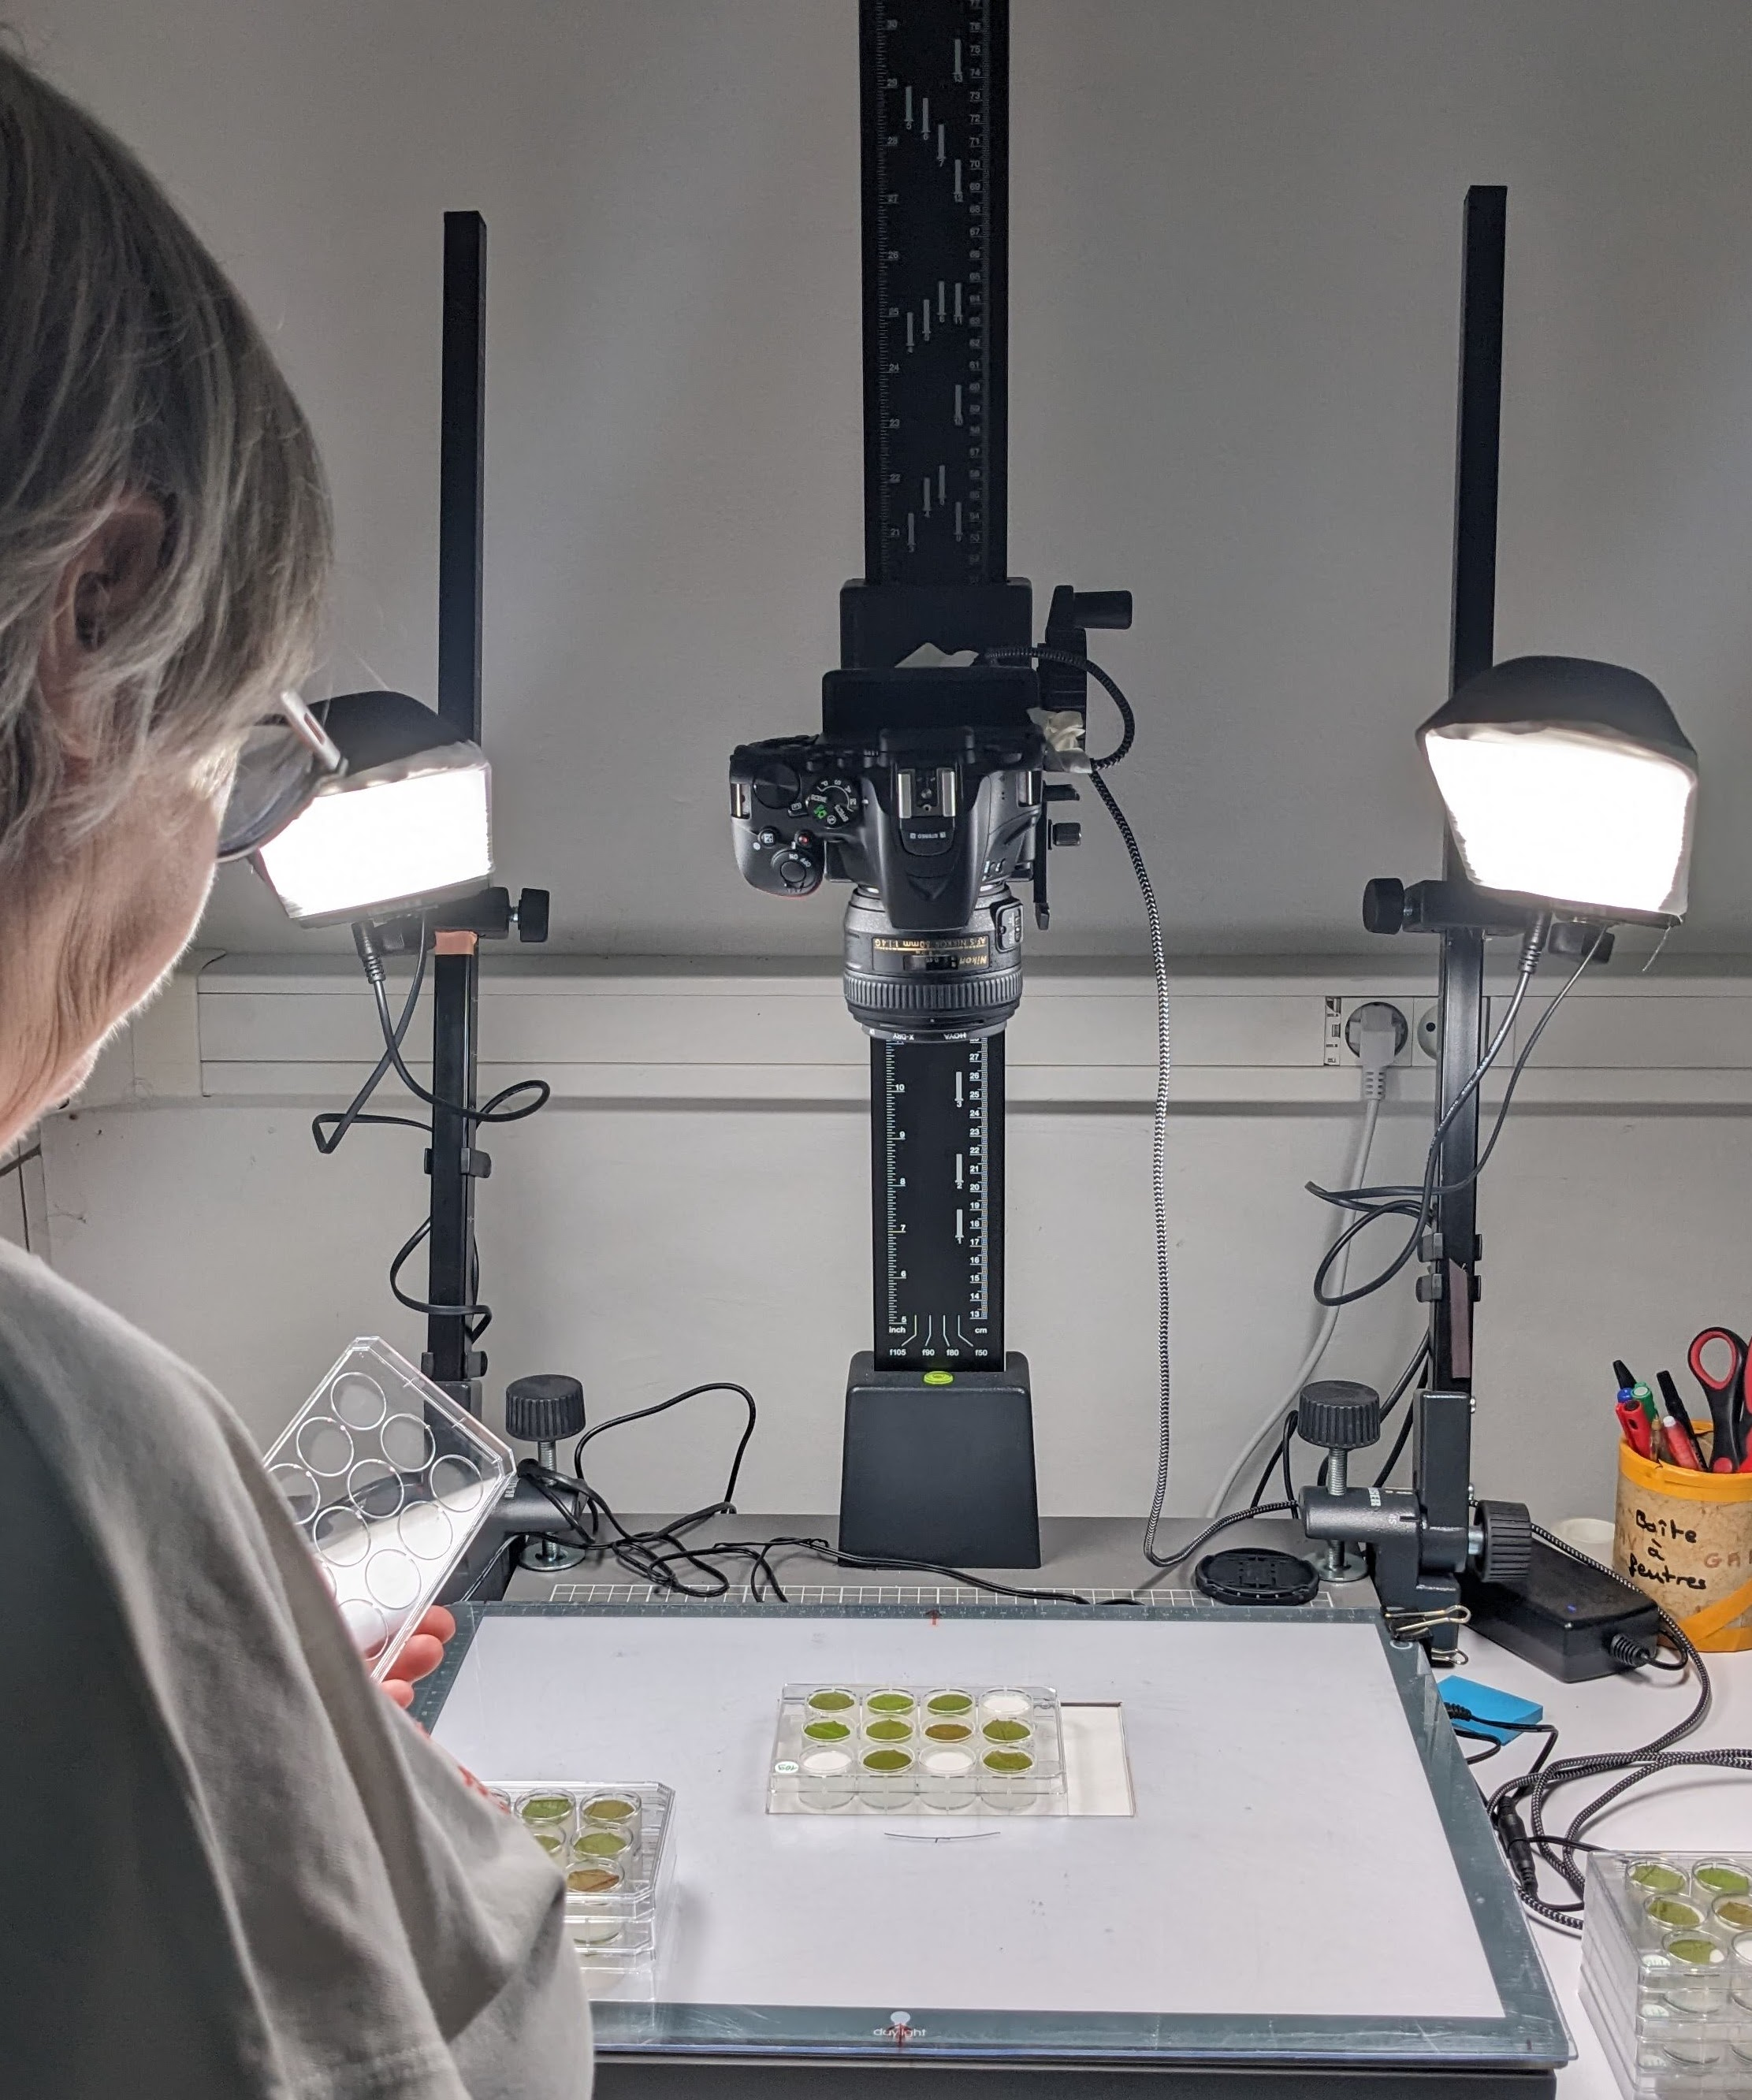
\includegraphics[width=0.5\linewidth]{2023_a_oiv_imaging_system.jpg}
        \caption{VEGOIA platform's manual imaging system}\label{fig:vegoia}
    \end{center}
\end{figure}

\begin{figure}[H]
    \centering
    \begin{subfigure}[b]{0.3\linewidth}
        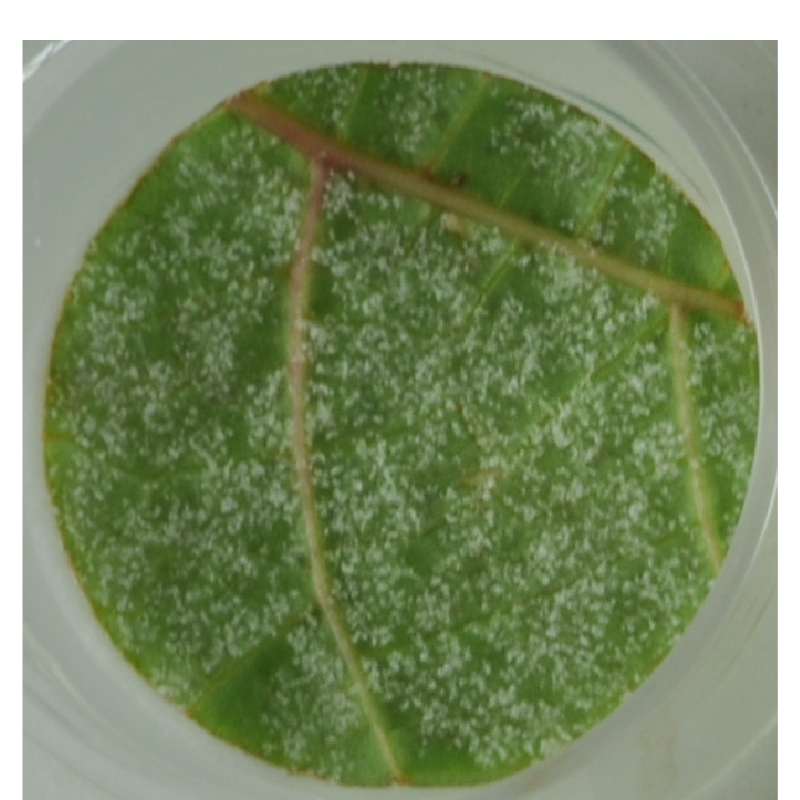
\includegraphics[width=\linewidth]{oiv1.png}
        \caption{OIV 1}\label{fig:oiv1}
    \end{subfigure}
    \begin{subfigure}[b]{0.3\linewidth}
        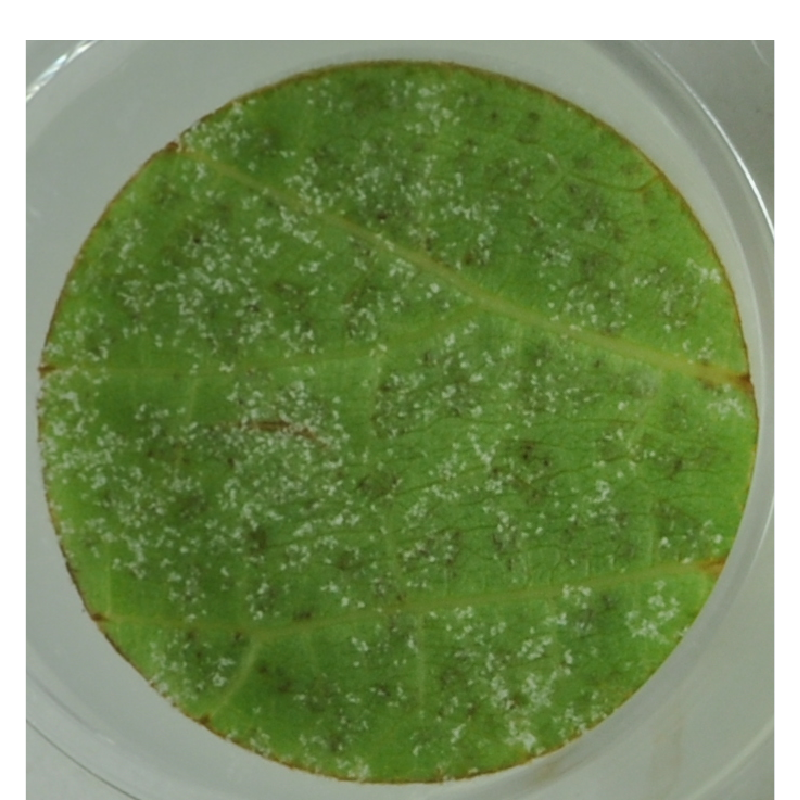
\includegraphics[width=\linewidth]{oiv3.png}
        \caption{OIV 3}\label{fig:oiv3}
    \end{subfigure}
    \begin{subfigure}[b]{0.3\linewidth}
        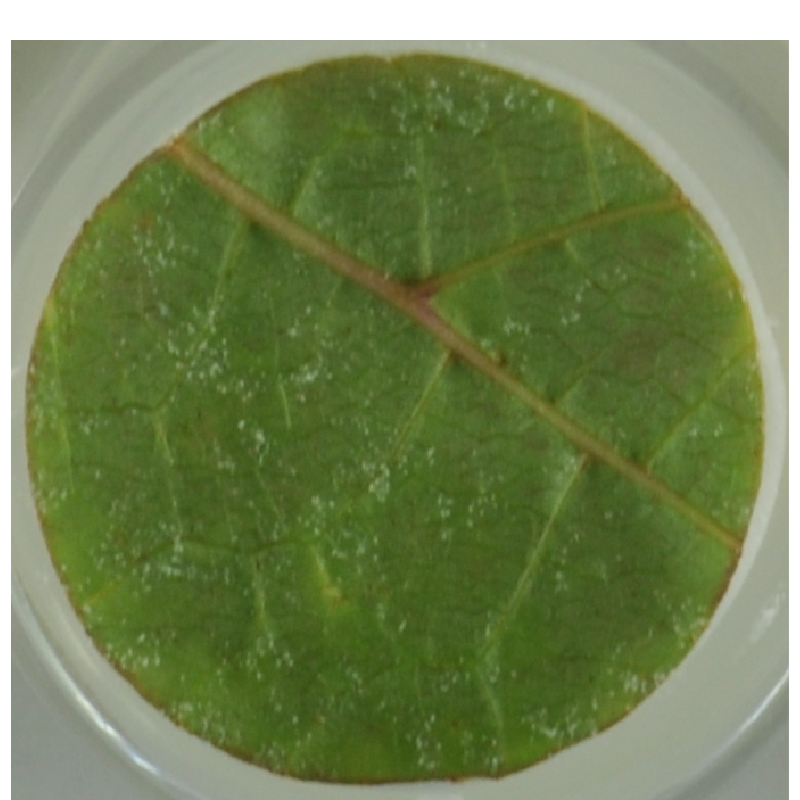
\includegraphics[width=\linewidth]{oiv5.png}
        \caption{OIV 5}\label{fig:oiv5}
    \end{subfigure}
    \begin{subfigure}[b]{0.3\linewidth}
        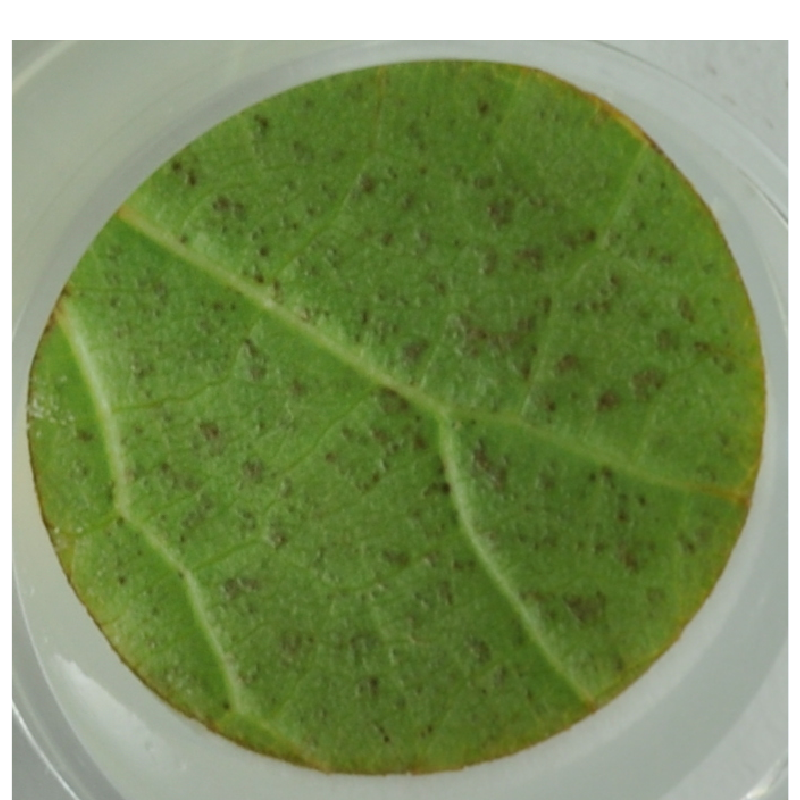
\includegraphics[width=\linewidth]{oiv7.png}
        \caption{OIV 7}\label{fig:oiv7}
    \end{subfigure}
    \begin{subfigure}[b]{0.3\linewidth}
        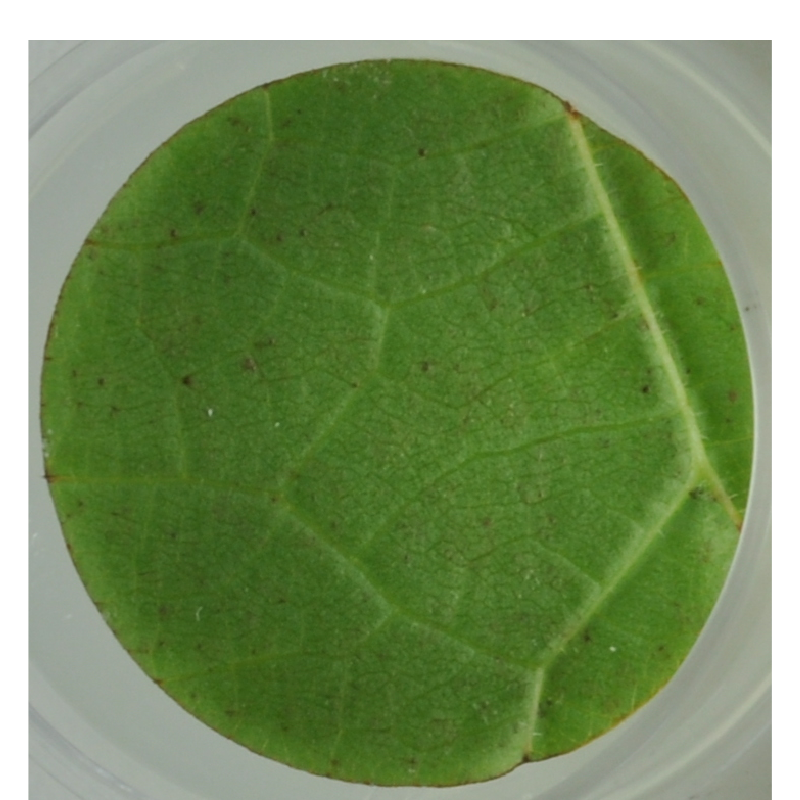
\includegraphics[width=\linewidth]{oiv9.png}
        \caption{OIV 9}\label{fig:oiv9}
    \end{subfigure}
    \caption{Exemples }\label{fig:phenotypes}
\end{figure}

\begin{figure}[H]
    \begin{center}
        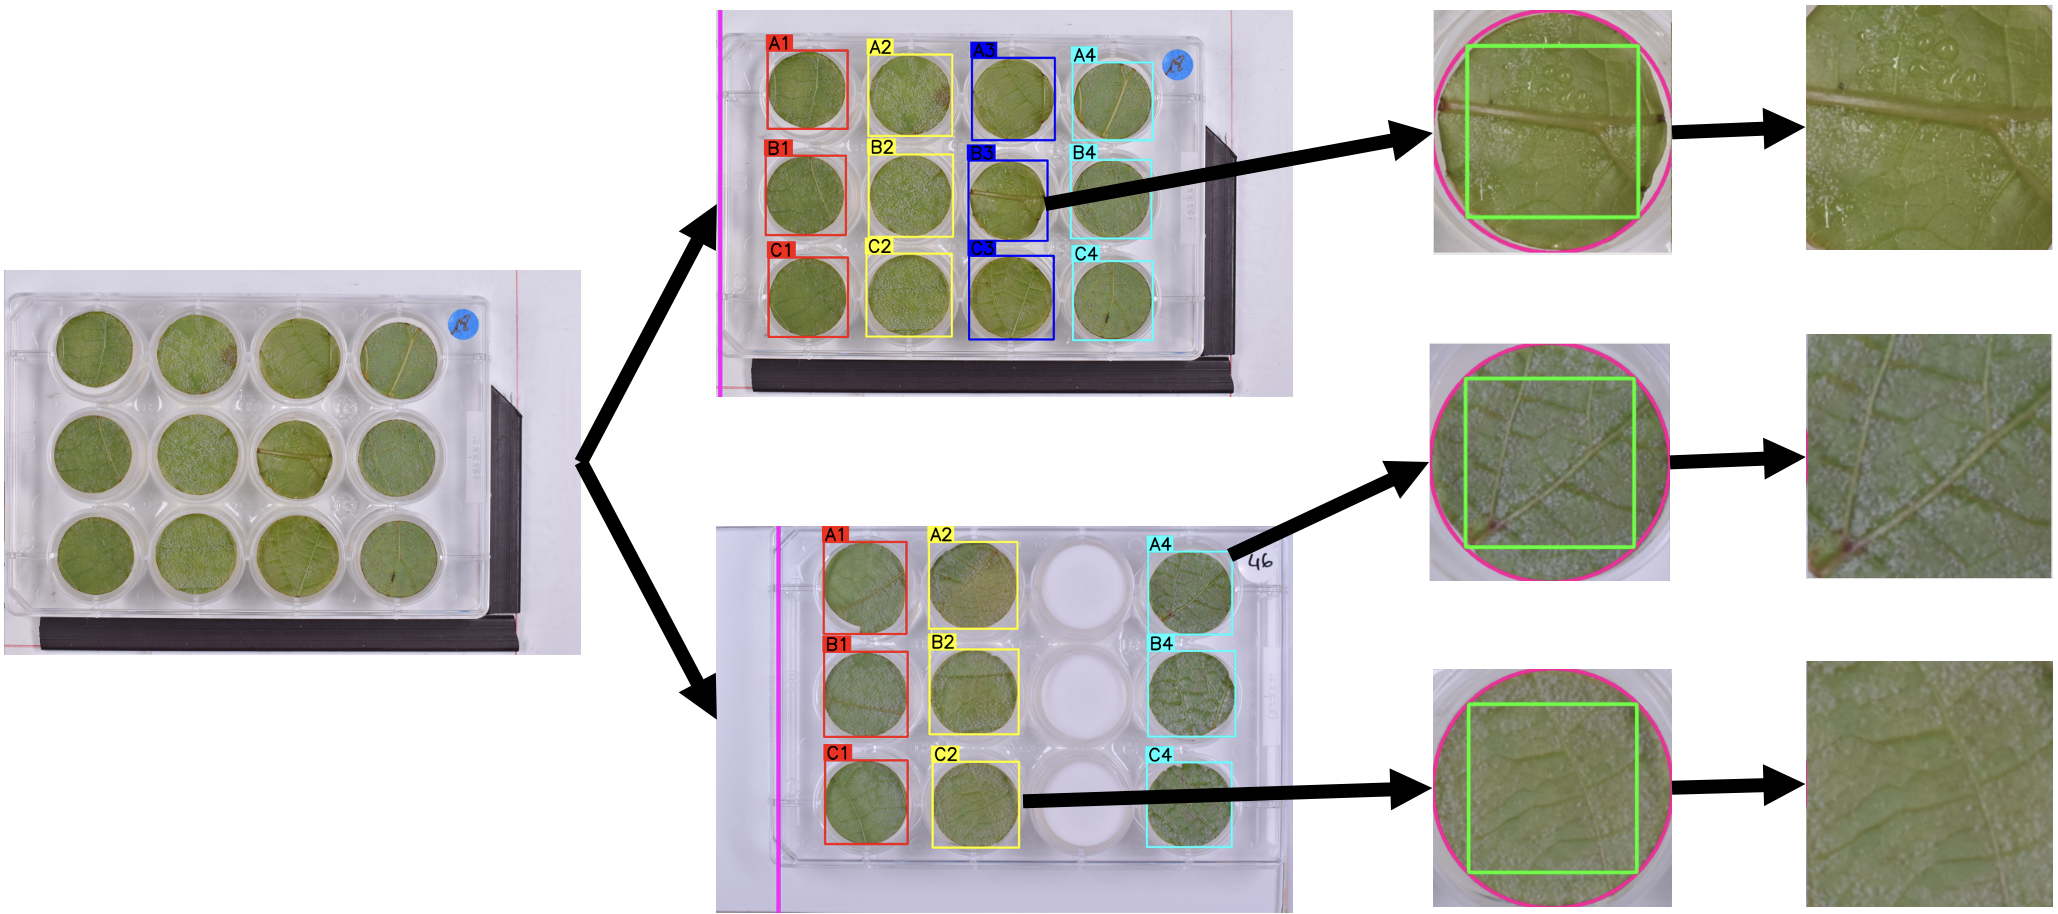
\includegraphics[width=0.9\linewidth]{2023_a_oiv_indexation}
        \caption{VEGOIA platform's manual imaging system}\label{fig:preprocessing}
    \end{center}
\end{figure}

\begin{figure}[H]
    \begin{center}
        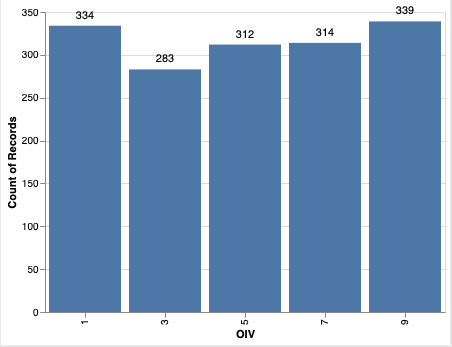
\includegraphics[width=0.7\linewidth]{2023_a_oiv_oiv_distribution}
        \caption{Dateset OIV distribution}\label{fig:datadistribution}
    \end{center}
\end{figure}


\section{Results and Discussion}


\begin{table}[H]
    \centering
    \caption{Average performance metrics with different ordinal regression metrics}
    \label{tab:dtafracevol}
    \begin{tabular}{llrrrrrrrr}
        \toprule
                           &            & \multicolumn{2}{l}{accuracy} & \multicolumn{2}{l}{f1 weighted avg} & \multicolumn{2}{l}{MSE} & \multicolumn{2}{l}{MAE}                                 \\
                           &            & mean                         & std                                 & mean                    & std                     & mean  & std   & mean  & std   \\
        Ordinal regression & backbone   &                              &                                     &                         &                         &       &       &       &       \\
        \midrule
        Naive              & pretrained & 0.775                        & 0.016                               & 0.769                   & 0.021                   & 0.229 & 0.018 & 0.227 & 0.016 \\
        coral              & pretrained & 0.447                        & 0.027                               & 0.368                   & 0.055                   & 0.737 & 0.052 & 0.612 & 0.024 \\
        corn               & pretrained & 0.778                        & 0.014                               & 0.772                   & 0.017                   & 0.224 & 0.015 & 0.223 & 0.014 \\
        spacecutter        & pretrained & 0.178                        & 0.003                               & 0.065                   & 0.011                   & 3.710 & 1.718 & 1.532 & 0.336 \\
        \bottomrule
    \end{tabular}
\end{table}

\begin{figure}[H]
    \begin{center}
        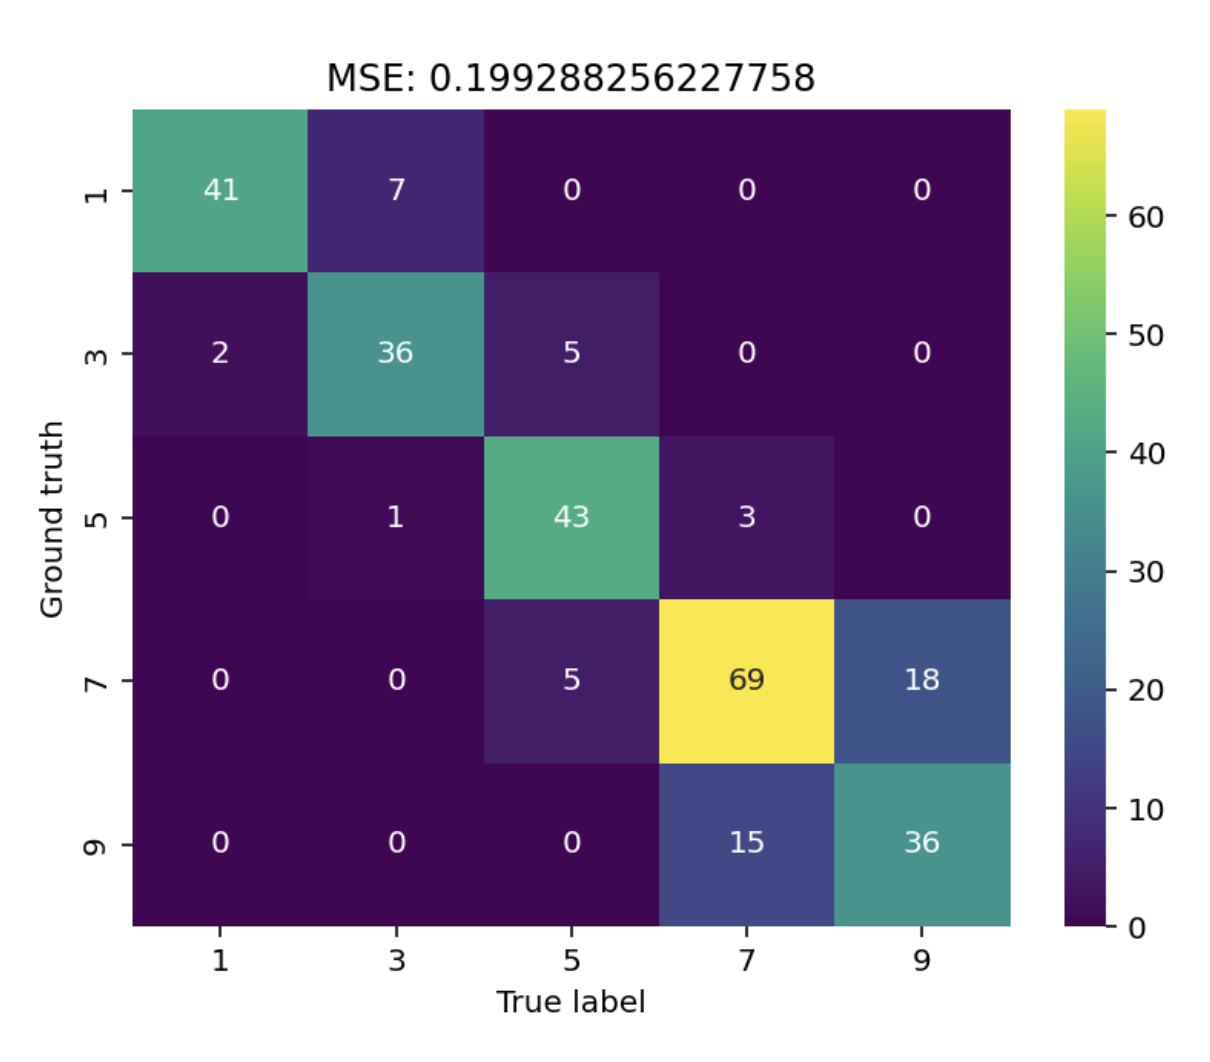
\includegraphics[width=0.7\linewidth]{2023_a_oiv_cm}
        \caption{Confusion matrix for best model using CORN ordinal regression method}\label{fig:oivcm}
    \end{center}
\end{figure}

\begin{table}[H]
    \centering
    \caption{Classification report}
    \label{tab:oivcr}
    \begin{tabular}{lrrrr}
        \toprule
        {}           & precision & recall & f1-score & support \\
        \midrule
        1            & 0.95      & 0.85   & 0.90     & 48      \\
        3            & 0.82      & 0.84   & 0.83     & 43      \\
        5            & 0.81      & 0.91   & 0.86     & 47      \\
        7            & 0.79      & 0.75   & 0.77     & 92      \\
        9            & 0.67      & 0.71   & 0.69     & 51      \\
                     &           &        &          &         \\
        accuracy     &           &        & 0.80     & 281     \\
        macro avg    & 0.81      & 0.81   & 0.81     & 281     \\
        weighted avg & 0.80      & 0.80   & 0.80     & 281     \\
        \bottomrule
    \end{tabular}
\end{table}

\section{Conclusions and perspectives}

% \begin{figure}[H]
%     \centering
%     \begin{subfigure}[b]{0.3\linewidth}
%         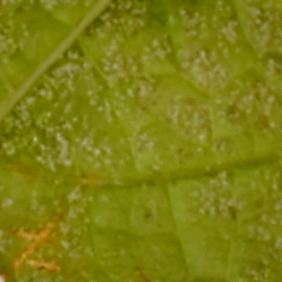
\includegraphics[width=\linewidth]{blur.png}
%         \caption{Blurred image}\label{fig:blurredimage}
%     \end{subfigure}
%     \begin{subfigure}[b]{0.3\linewidth}
%         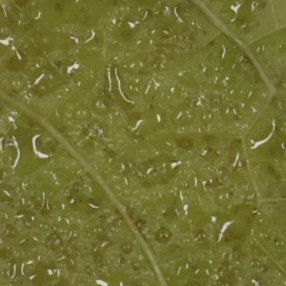
\includegraphics[width=\linewidth]{water.png}
%         \caption{Water droplets}\label{fig:waterimage}
%     \end{subfigure}
%     \begin{subfigure}[b]{0.3\linewidth}
%         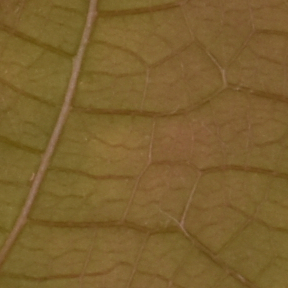
\includegraphics[width=\linewidth]{color.png}
%         \caption{Innate color issue}\label{fig:colorimage}
%     \end{subfigure}
%     \caption{Images with issues are hard to predict by the model}\label{fig:badimages}
% \end{figure}

\begin{figure}[H]
    \centering
    \begin{subfigure}[b]{0.45\linewidth}
        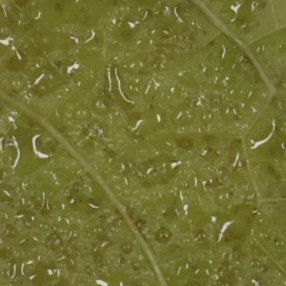
\includegraphics[width=\linewidth]{water.png}
        \caption{Water droplets may be mistaken with sporulation}\label{fig:error97water}
    \end{subfigure}
    \begin{subfigure}[b]{0.45\linewidth}
        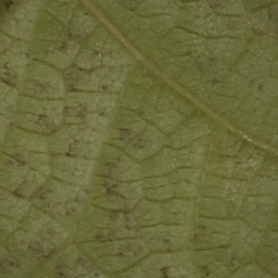
\includegraphics[width=\linewidth]{error_97.png}
        \caption{White stains appear in image}\label{fig:error97b}
    \end{subfigure}
    \caption{Images with OIV value 9 predicted as 7}\label{fig:errors97}
\end{figure}

\begin{figure}[H]
    \centering
    \begin{subfigure}[b]{0.45\linewidth}
        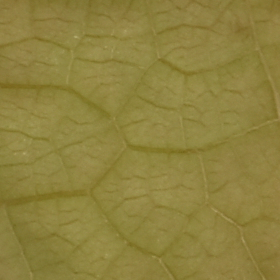
\includegraphics[width=\linewidth]{error_79_2.png}
        \caption{}\label{fig:error79a}
    \end{subfigure}
    \begin{subfigure}[b]{0.45\linewidth}
        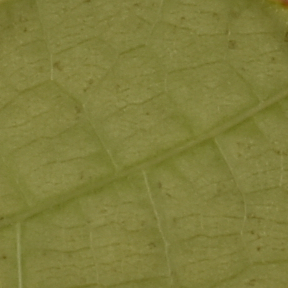
\includegraphics[width=\linewidth]{error_79_1.png}
        \caption{}\label{fig:error79b}
    \end{subfigure}
    \caption{Images with OIV value 7 predicted as 9 when sporulation is hardly perceptible}\label{fig:errors79}
\end{figure}


\end{document}